%UNIT 6: AUTONOMOUS DIFFERENTIAL EQUATIONS
%%%%%%%%%%%%%%%%%%%%%%%%%%%
%%%% Put the following at the top of each .tex file  %
\pagestyle{fancy}
\renewcommand{\theUnit}{1.6}
\ifthenelse{\isundefined{\UnitPageNumbers}}{}{\setcounter{page}{1}}
\rhead{Section \theUnit: Autonomous Equations and Phase Diagrams}
\lhead{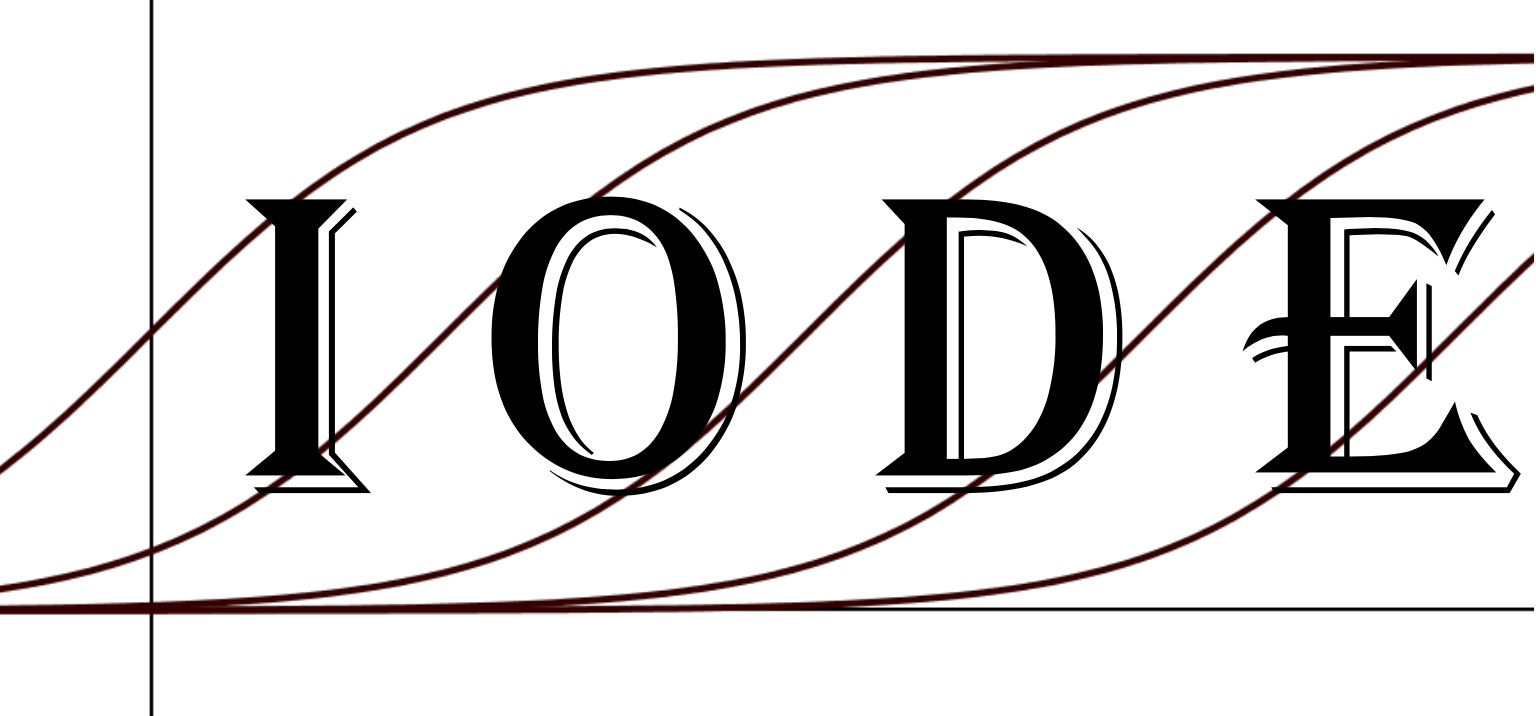
\includegraphics[width=1.25cm]{IODE-logo.png}}
\rfoot{\mypage}
\lfoot{}
\cfoot{}
\fancypagestyle{firstfooter}{\footskip = 50pt}
\renewcommand{\footrulewidth}{.4pt}
%%%%%%%%%%%%%%%%%%%%%%%%%%%
\vspace*{-20pt} \thispagestyle{firstfooter}
\pagebegin{Analyzing Autonomous DEs: Spotted Owls}

A group of biologists are making predictions about the spotted owl population in a forest in the Pacific Northwest.  The autonomous differential equation the scientist use to model the spotted owl population is $\displaystyle \frac{dP}{dt}=\frac{P}{2}\left(1-\frac{P}{5}\right)\left(\frac{P}{8}-1\right)$, where $P$ is in hundreds of owls and $t$ is in years. The problem is that the current number of owls is only approximately known.  
\begin{enumerate}
\item Suppose the scientists estimate that currently $P$ is about 5 (i.e. there are currently about 500 owls in the forest).  Since 5 is only an estimate, they make long-term predictions of the owl population for the initial conditions $P = 4.9$, $P = 5.0$, and $P = 5.1$. \textit{Without using a graphing calculator or other software}, determine the long-term predictions for these initial conditions based on the differential equation. Are they similar or different?  That is, will slightly different initial conditions yield only slightly different long-term predictions, or will they be radically different? Carry out a similar analysis if the current number of owls is somewhere around 8.\label{04problem1}
\vspace{4in}

\item Give a one dimensional representation, \textit{without words}, that would describe all solutions to the differential equation. \label{04problem2}

\clearpage
\item A \textbf{phase line} is the standard one-dimensional diagram that depicts the qualitative behavior of solutions to an autonomous differential equation. Label the dots and add arrows to the figure below to represent \textbf{all} solutions to the differential equation in Problem \ref{04problem1}. \label{04problem3} \\
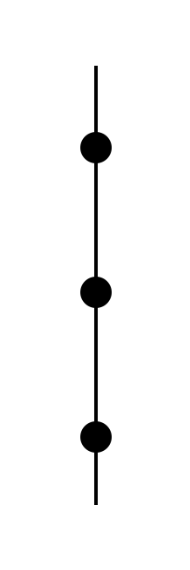
\includegraphics[width=1in]{04/04PhaseLine.png}

\item For the differential equation in problems \ref{04problem1}-\ref{04problem3} there are three equilibrium solutions. Recall that equilibrium solutions are constant functions that satisfy the differential equation. How do the other solution functions near each equilibrium solution behave in the long term? If you were to label each of these equilibrium solutions based on the way in which nearby solutions behave, what terms would you use and why? \label{04problem4} 

\end{enumerate}

\clearpage

%\pagebegin{Phase Lines}

\begin{enumerate}[resume]
%\item Dominique is working with the rate of change equation $\frac{dP}{dt}=0.2P$  and thinks about solutions in terms of whether they are increasing, decreasing, or remaining constant. She illustrates her thinking with the phase line shown below. 
%\begin{center}
%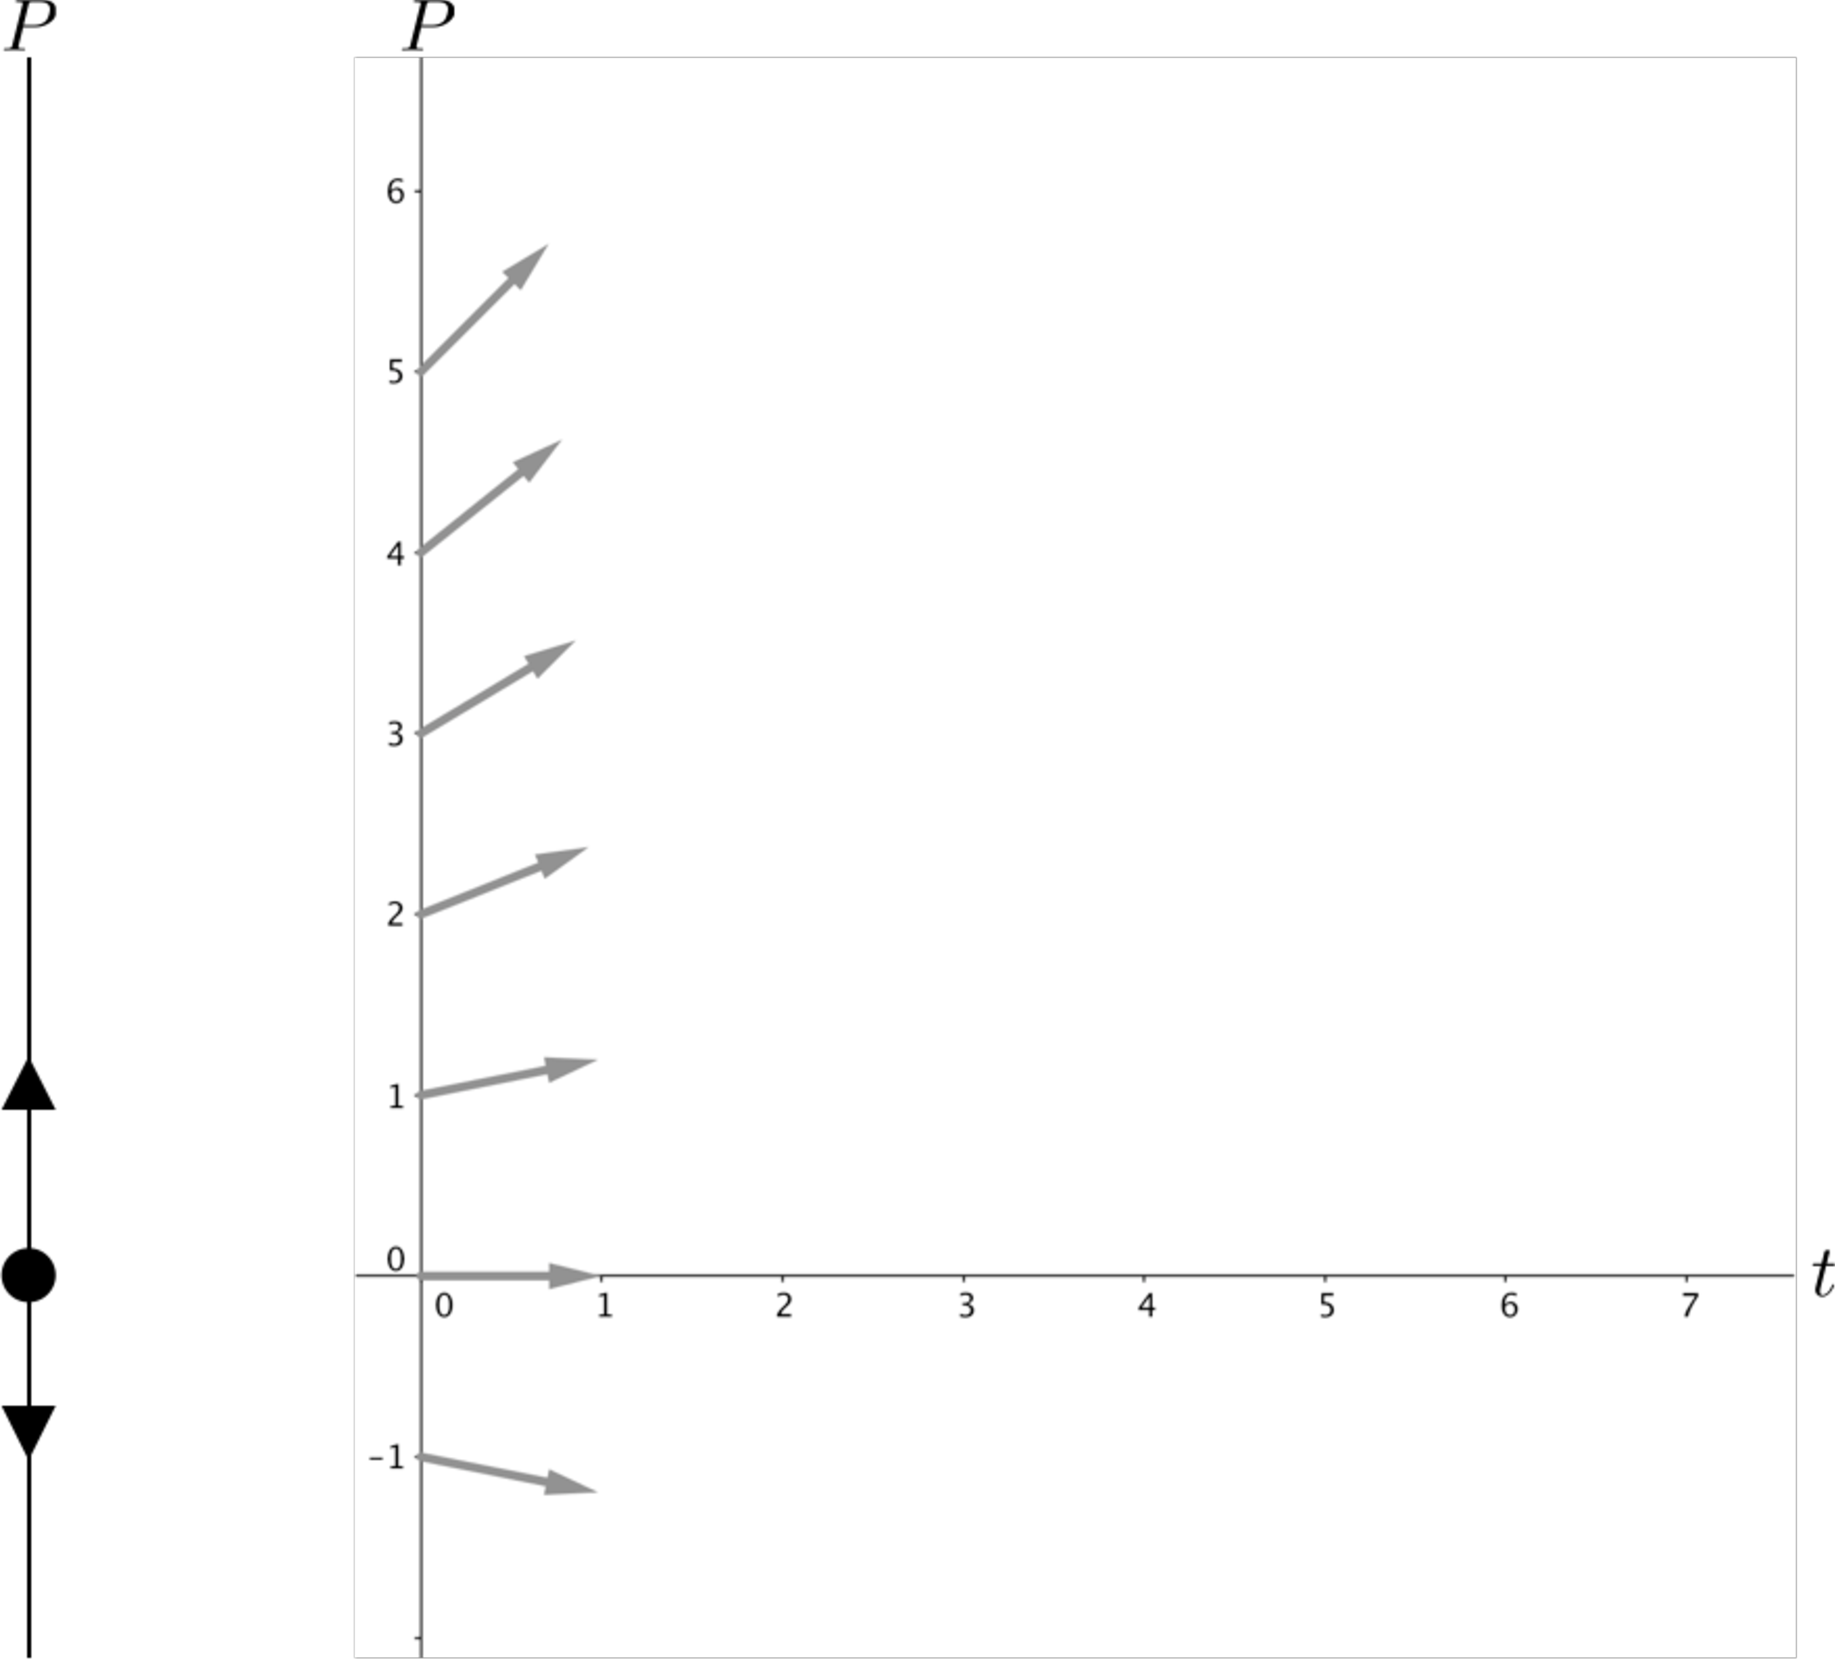
\includegraphics[width=6in]{04/04PhaseLineAndSomeVectors.pdf} \\
%\end{center}
%\clearpage
%\begin{enumerate}
%\item	Place your fingertip or other small item on the phase line at $P = 0$ and another fingertip or small item at $P = 0$ on the $P$ vs $t$ axes and imagine time moving forward. Explain, with reasons, what happens to your fingertips. \label{04problem5parta} \vfill

%\item	Place your fingertip or other small item on the phase line at $P = 1$ and another fingertip or small item at $P = 1$ on the $P$ vs $t$ axes at (0,1) and imagine time moving forward. Explain, with reasons, what happens to your fingertips. \label{04problem5partb}   \vfill

%\item	Place two fingertips or two small items on the phase line, one at $P = 1$ and the other at $P = 3$. What happens to your fingertips as time moves forward? How do your ideas relate to the corresponding $P$ versus $t$ graphs? \label{04problem5partc}  \vfill

%\item	Explain how a person could think about the phase line as a one-dimensional projection of all of the two-dimensional $P(t)$ graphs of solutions. \label{04problem5partd} \vfill

%\end{enumerate}

\item Create an autonomous differential equation that has exactly two equilibrium solutions: $y(t)=3$ is a stable equilibrium and $y(t) = -4$ is an unstable equilibrium.

\end{enumerate}
\clearpage

%%%%%%%%%%%%%%%%%%%%%%%%%%%%%%%%%%%%%%%%%%%%%%%%%%%%%%%%%%%%%%%%%%%%%%%%%%%%%%%%%%%%%%%%%%
\pagebegin{Homework Set 4}

\begin{enumerate}
\item For an autonomous differential equations, it is possible to view all of the solution function graphs in terms of ``prototypical'' graphs. A prototypical solution graph represents an infinite number of other solution graphs. For example, in part (i) below one can view the entire family of functions that solve the differential equation in terms of two different prototypical solution graphs separated by an equilibrium solution: one prototypical solution graph is above the $t$-axis and one is below the $t$-axis. Each is prototypical because it can stand for all other solution graphs (in its respective region) through horizontal translation. Recall the ``Making Connections'' section of Unit 3. \label{04HWproblem1}
\begin{hnumerate}
\hitem    $\displaystyle\frac{dy}{dt}=-y$    \hitem $\displaystyle\frac{dy}{dt}=2y\left(1-\frac{y}{2}\right)$        \hitem $\displaystyle\frac{dy}{dt}=2y\left(1-\frac{y}{2}\right)+3$        \hitem   $\displaystyle\frac{dy}{dt}=y^2$ \end{hnumerate}
\begin{enumerate}
\item For each differential equation above, draw a phase line and representative graphs of solutions. \label{04HWproblem1parta}
\item For each differential equation above, explain how your response to number \ref{04HWproblem1parta} can be interpreted in terms of prototypical solutions separated by equilibrium solutions. \label{04HWproblem1partb} 
\end{enumerate}

\item For each of the following slope fields, create a differential equation whose slope field would be similar to the one given. Give reasons for why you created the differential equation as you did. You may create whatever scale on the axes that you want. \label{04HWproblem2} \\
\begin{enumerate*}
\item 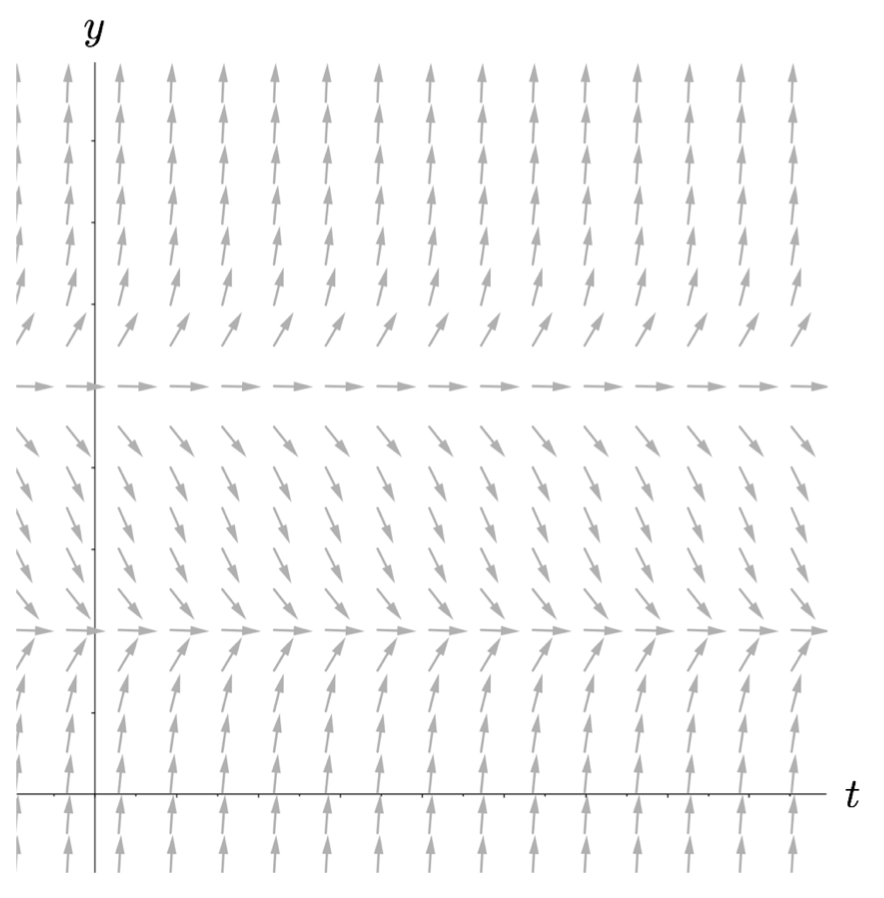
\includegraphics[width=3in]{04/04HWSlopeFieldA.png}
\item 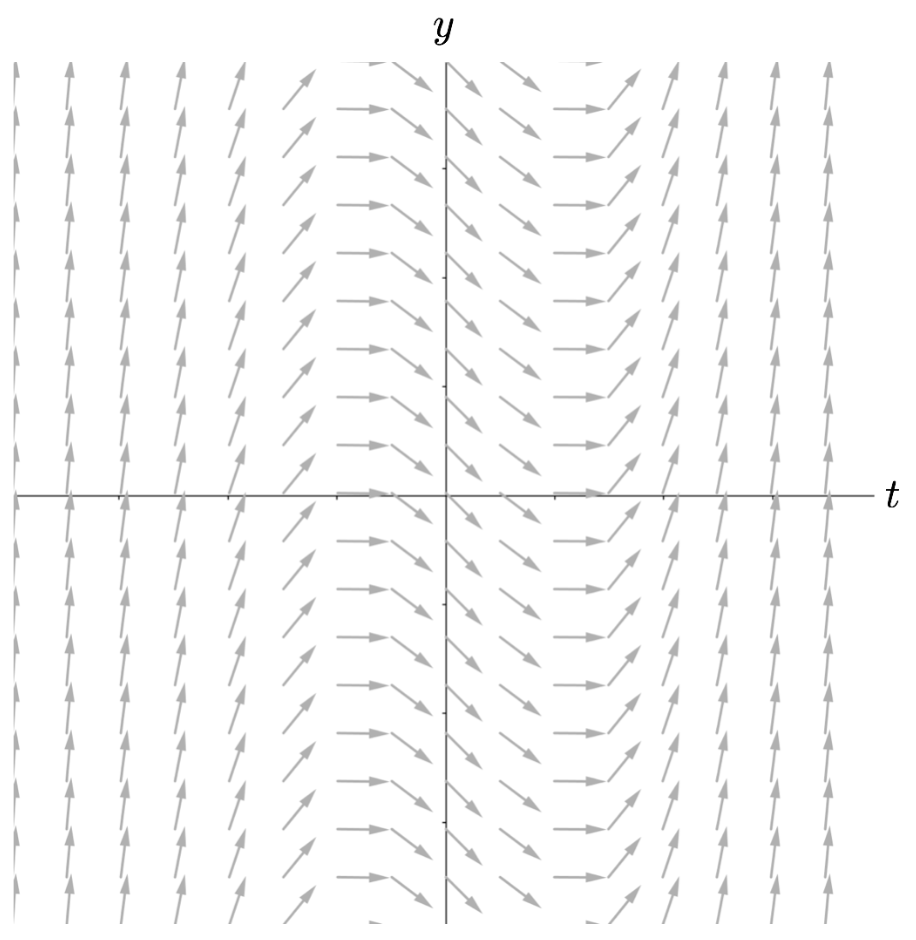
\includegraphics[width=3in]{04/04HWSlopeFieldB.png}
\item 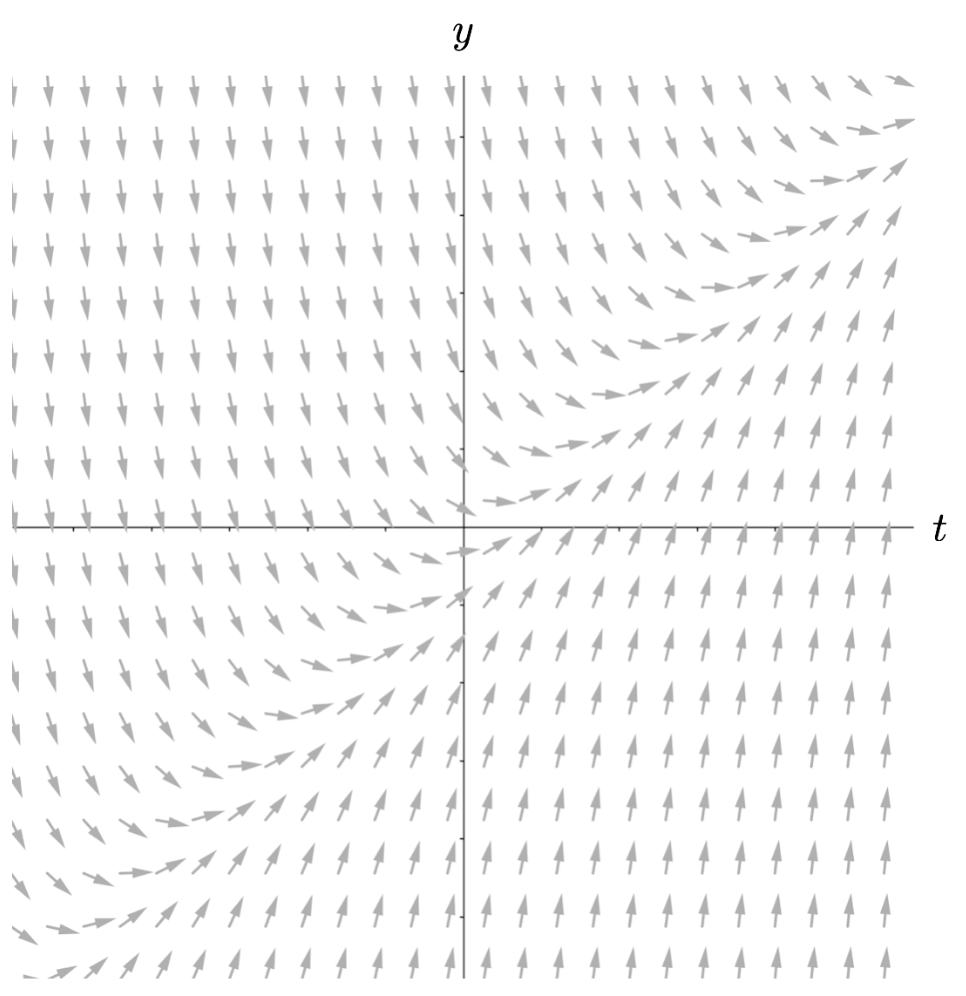
\includegraphics[width=3in]{04/04HWSlopeFieldC.png}
\item 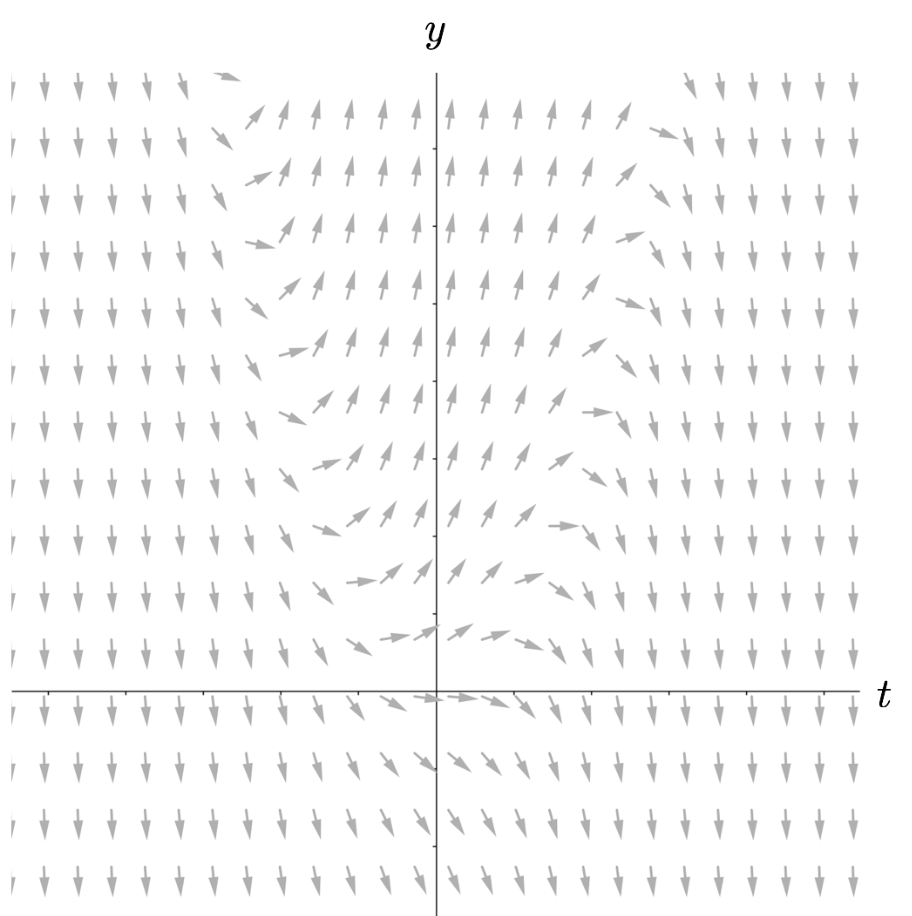
\includegraphics[width=3in]{04/04HWSlopeFieldD.png}
\end{enumerate*}

\item For each part below, create a continuous, autonomous differential equation that has the stated properties (if possible). Explain how you created each differential equation and include all graphs or diagrams you used and how you used them. If it is not possible to come up with a differential equation with the stated properties, provide a justification for why it cannot be done. \label{04HWproblem3}

\begin{enumerate}
\item Exactly three constant solution functions, two repellers and one attractor.
\item	Exactly two constant solution functions, one a repeller and one a node.
\item	Exactly two constant solution functions, both attractors.
\end{enumerate}

\item For each part below, create an autonomous differential equation that satisfies the stated criteria \label{04HWproblem4}
\begin{enumerate}
\item	$y(t)=0$ and $y(t) = -4$ are the only constant solution functions
\item $y(t)=e^{-t+1}$ is a solution
\item $y(t)=e^{2t-5}$	is a solution
\item $y(t)=10e^{0.3t}$ is a solution
\item $y(t)=1-e^{-t}$ and $y(t)=1+e^{-t}$ are solutions
\end{enumerate}

\item For a phase line to be a meaningful tool, explain why it is essential for the differential equation to be autonomous. \label{04HWproblem5}

\item In class you and your classmates continue to develop creative and effective ways of thinking about particular ideas or problems. Discuss at least one idea or way of thinking about a particular problem that has been discussed in class (either in whole class discussion or in small group) that was particularly helpful for enlarging your own thinking and/or that you disagreed with and had a different way of thinking about the idea or problem. \label{04HWproblem6}

\end{enumerate}
